% Figure: FlashAttention changes which tensors are materialised in which memory,
% and therefore how many bytes cross the HBM boundary.  Design width ~168mm.
\documentclass[border=0pt]{standalone}
\usepackage{amsmath,amssymb}
% Shared visual language for the figures of the book.
% Every figure in this directory loads this file so the chapter reads as one system.
% NOTE: no blank lines are allowed inside \tikzset{...} (a blank line emits \par
% and breaks key scanning).
\NeedsTeXFormat{LaTeX2e}
\ProvidesPackage{figstyle}[2026/10/21 Figure style for Free Energy to LLMs]

\RequirePackage{tikz}
\usetikzlibrary{arrows.meta,positioning,calc,fit,shapes.geometric,shapes.misc,%
  backgrounds,matrix,decorations.pathreplacing,decorations.markings,patterns.meta}

% ---------------------------------------------------------------- palette
% Same values as book/preamble/style.tex, prefixed with F.
\definecolor{FNavy}{HTML}{14324A}
\definecolor{FTeal}{HTML}{0E7490}
\definecolor{FSky}{HTML}{E7F5F8}
\definecolor{FOrange}{HTML}{D97706}
\definecolor{FAmber}{HTML}{FFF3D6}
\definecolor{FInk}{HTML}{1F2937}
\definecolor{FSlate}{HTML}{64748B}
\definecolor{FMist}{HTML}{F5F7FA}
\definecolor{FRose}{HTML}{9F1239}
\definecolor{FRoseMist}{HTML}{FFF1F2}

% ---------------------------------------------------------------- semantics
% Teal   = probability / model / data object
% Orange = training objective, cost, or the quantity moved through the system
% Navy   = neutral structure
% Slate  = secondary label or metadata
% Rose   = failure mode, hazard, masked-out region
\tikzset{
  % Lay figures out in millimetres.  A figure designed 168mm wide is included at
  % \textwidth, so its fonts appear at exactly the size written here.
  every picture/.style={x=1mm,y=1mm,font=\small,line cap=round,line join=round},
  % ---- block styles
  nbase/.style={draw,rounded corners=1.2pt,align=center,inner sep=2.4pt,%
    minimum height=7mm,text=FInk},
  nteal/.style={nbase,draw=FTeal,fill=FSky},
  norange/.style={nbase,draw=FOrange,fill=FAmber},
  nnavy/.style={nbase,draw=FNavy,fill=white},
  nsoft/.style={nbase,draw=FSlate!55,fill=FMist},
  nrose/.style={nbase,draw=FRose,fill=FRoseMist},
  ghost/.style={draw=none,fill=none,align=center,inner sep=1pt},
  plain/.style={draw=none,fill=none,align=center,inner sep=0pt},
  % ---- arrows
  ar/.style={-{Latex[length=1.7mm,width=1.35mm]},draw=FSlate,line width=0.75pt},
  ard/.style={ar,dashed},
  arteal/.style={ar,draw=FTeal},
  arorange/.style={ar,draw=FOrange},
  arrose/.style={ar,draw=FRose},
  thickar/.style={ar,line width=1.2pt},
  % ---- text roles
  ftitle/.style={font=\large\bfseries,text=FNavy,align=center},
  ptitle/.style={font=\small\bfseries,text=FNavy,align=center},
  ptitleo/.style={font=\small\bfseries,text=FOrange,align=center},
  lbl/.style={font=\scriptsize,text=FSlate,align=center,inner sep=1pt},
  lblt/.style={lbl,text=FTeal},
  lblo/.style={lbl,text=FOrange},
  lbln/.style={lbl,text=FNavy},
  lblr/.style={lbl,text=FRose},
  sub/.style={font=\scriptsize,text=FSlate!90,align=center,inner sep=1pt},
  monob/.style={font=\ttfamily\scriptsize,text=FInk,inner sep=1pt},
  mathb/.style={font=\small,text=FInk,inner sep=1pt},
  eqn/.style={font=\scriptsize,inner sep=1.5pt,text=FInk},
  % ---- decorations
  brace/.style={decorate,decoration={brace,amplitude=2.4pt},draw=FSlate,%
    line width=0.6pt},
  bracet/.style={brace,draw=FTeal},
  braceo/.style={brace,draw=FOrange},
  axis/.style={draw=FSlate!55,line width=0.6pt},
  guide/.style={draw=FSlate!45,line width=0.5pt,dashed},
  halolabel/.style={font=\scriptsize,text=FInk,fill=white,fill opacity=0.85,%
    text opacity=1,inner sep=1.4pt,align=center},
}

% Figure title above the drawing, anchored at the figure's top-left.
\newcommand{\figtitle}[2][0]{%
  \node[ftitle,anchor=north west,outer sep=0pt] at (#1,0) {#2};}

% Rounded panel behind a subgroup of nodes.
\newcommand{\figpanel}[3][]{%
  \node[draw=FSlate!35,fill=#3,rounded corners=2pt,inner sep=2.6mm,#1] {#2};}

\endinput

\begin{document}
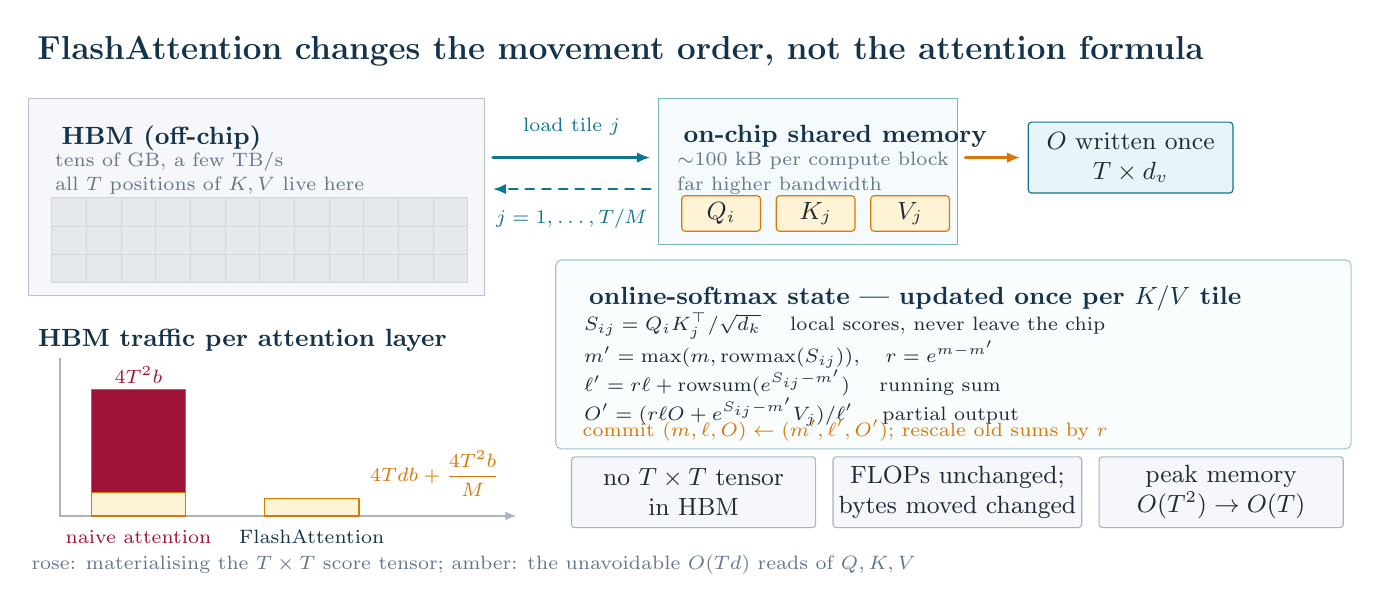
\begin{tikzpicture}
\figtitle{FlashAttention changes the movement order, not the attention formula}
% ------------------------------------------------------------- HBM level
\draw[draw=FSlate!45,fill=FMist] (0,-34) rectangle (58,-9);
\node[ptitle,anchor=north west] at (3,-11.2) {HBM (off-chip)};
\node[lbl,anchor=north west] at (3,-15.4) {tens of GB, a few TB/s};
\node[lbl,anchor=north west] at (3,-18.6) {all $T$ positions of $K,V$ live here};
\foreach \cx in {0,...,11}{%
  \foreach \ry in {0,...,2}{%
    \draw[draw=FSlate!30,fill=FSlate!16,line width=0.3pt]%
      (3+4.4*\cx,-21.6-3.6*\ry) rectangle ++(4.4,-3.6);}}
% ---------------------------------------------------------- SRAM level
\draw[draw=FTeal!55,fill=FSky!40] (80,-27.5) rectangle (118,-9);
\node[ptitle,anchor=north west] at (82,-11.2) {on-chip shared memory};
\node[lbl,anchor=north west] at (82,-15.4) {$\sim$100 kB per compute block};
\node[lbl,anchor=north west] at (82,-18.6) {far higher bandwidth};
\foreach \tx/\tl in {83/$Q_i$,95/$K_j$,107/$V_j$}{%
  \node[norange,minimum width=10mm,minimum height=4.5mm,inner sep=0pt] at (\tx+5,-23.6) {\tl};}
% -------------------------------------------------------------- IO arrows
\node[lblt] at (69,-12.6) {load tile $j$};
\draw[arteal,line width=1pt] (59,-16.5)--(79,-16.5);
\draw[arteal,dashed,line width=1pt] (79,-20.5)--(59,-20.5);
\node[lblt] at (69,-24.2) {$j=1,\dots,T/M$};
% ------------------------------------------------------------- output box
\draw[arorange,line width=1pt] (119,-16.5)--(126,-16.5);
\node[nteal,minimum width=26mm,minimum height=9mm,inner sep=2.4pt] at (140,-16.5)
  {$O$ written once\\$T\times d_v$};
% ----------------------------------------------- online softmax state
\draw[draw=FTeal!40,fill=FSky!22,rounded corners=2pt] (67,-53.5) rectangle (168,-29.5);
\node[ptitle,anchor=north west] at (70,-31.6)
  {online-softmax state --- updated once per $K/V$ tile};
\node[eqn,anchor=north west] at (70,-35.6)
  {$S_{ij}=Q_iK_j^{\top}/\sqrt{d_k}$ \quad local scores, never leave the chip};
\node[eqn,anchor=north west] at (70,-39.2)
  {$m^{\prime}=\max(m,\mathrm{rowmax}(S_{ij})),\quad r=e^{m-m^{\prime}}$};
\node[eqn,anchor=north west] at (70,-42.8)
  {$\ell^{\prime}=r\ell+\mathrm{rowsum}(e^{S_{ij}-m^{\prime}})$ \quad running sum};
\node[eqn,anchor=north west] at (70,-46.4)
  {$O^{\prime}=(r\ell O+e^{S_{ij}-m^{\prime}}V_j)/\ell^{\prime}$ \quad partial output};
\node[lblo,anchor=north west] at (70,-49.4)
  {commit $(m,\ell,O)\leftarrow(m^{\prime},\ell^{\prime},O^{\prime})$; rescale old sums by $r$};
% ----------------------------------------- result strip
\node[nsoft,minimum width=31mm,minimum height=9mm,inner sep=2pt] at (84.5,-59)
  {no $T\times T$ tensor\\in HBM};
\node[nsoft,minimum width=31mm,minimum height=9mm,inner sep=2pt] at (118,-59)
  {FLOPs unchanged;\\bytes moved changed};
\node[nsoft,minimum width=31mm,minimum height=9mm,inner sep=2pt] at (151.5,-59)
  {peak memory\\$O(T^2)\rightarrow O(T)$};
% ------------------------------------------- before / after HBM traffic
\node[ptitle,anchor=north west] at (0,-37) {HBM traffic per attention layer};
\draw[axis] (4,-62)--(4,-42);
\draw[axis,-{Latex[length=1.4mm,width=1.1mm]}] (4,-62)--(62,-62);
\draw[fill=FRose,draw=FRose!70,line width=0.4pt] (8,-59)--(8,-46)--(20,-46)--(20,-59);
\draw[fill=FAmber,draw=FOrange,line width=0.5pt] (8,-62) rectangle (20,-59);
\draw[fill=FRose,draw=FRose!70,line width=0.4pt] (30,-60.2)--(30,-59.8)--(42,-59.8)--(42,-60.2);
\draw[fill=FAmber,draw=FOrange,line width=0.5pt] (30,-62) rectangle (42,-59.8);
\node[lblr,anchor=south] at (14,-45.6) {$4T^2b$};
\node[lblo,anchor=west] at (43,-56.6) {$4Tdb+\dfrac{4T^2b}{M}$};
\node[lblr,anchor=north] at (14,-63.4) {naive attention};
\node[lbln,anchor=north] at (36,-63.4) {FlashAttention};
\node[lbl,anchor=north west] at (0,-66.6)
  {rose: materialising the $T\times T$ score tensor; amber: the unavoidable $O(Td)$ reads of $Q,K,V$};
\end{tikzpicture}
\end{document}
